Git jest bardzo popularnym, potężnym i wydajnym systemem kontroli wersji Open Source, który śledzi treści takie jak pliki i katalogi. Jego głównym celem jest zarządzanie projektem lub zestawem plików w miarę ich zmian w czasie.

System kontroli wersji, czyli VCS, jak to się powszechnie określa, jest systemem, który śledzi historię zmian, gdy ludzie i zespoły współpracują ze sobą nad projektami. W miarę jak projekt ewoluuje, zespoły mają możliwość przeprowadzania testów, usuwania błędów i tworzenia nowego kodu z pewnością, że każda wersja może zostać odzyskana w dowolnym momencie.

\begin{figure}[H]
    \centering
    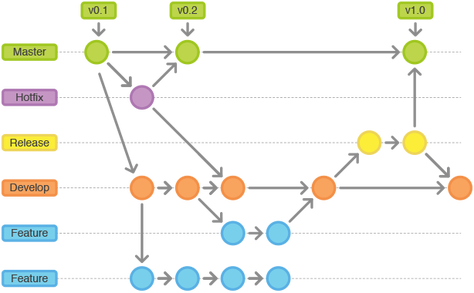
\includegraphics[width=6in]{images/git.png}
    \caption{Przykładowy układ na zasadzie git flow ze strony https://barloblog.wordpress.com \label{fig:git}}
\end{figure}